\section{Thiết kế giao diện người dùng (UI)}
Phần này trình bày 22 hình ảnh giao diện thực tế của hệ thống LumiCinema kèm theo \textbf{Danh sách thành phần} và \textbf{Danh sách biến cố} tương ứng cho từng màn hình chính.

\subsection{Giao diện Trang chủ LumiCinema}
\begin{figure}[H]
  \centering
  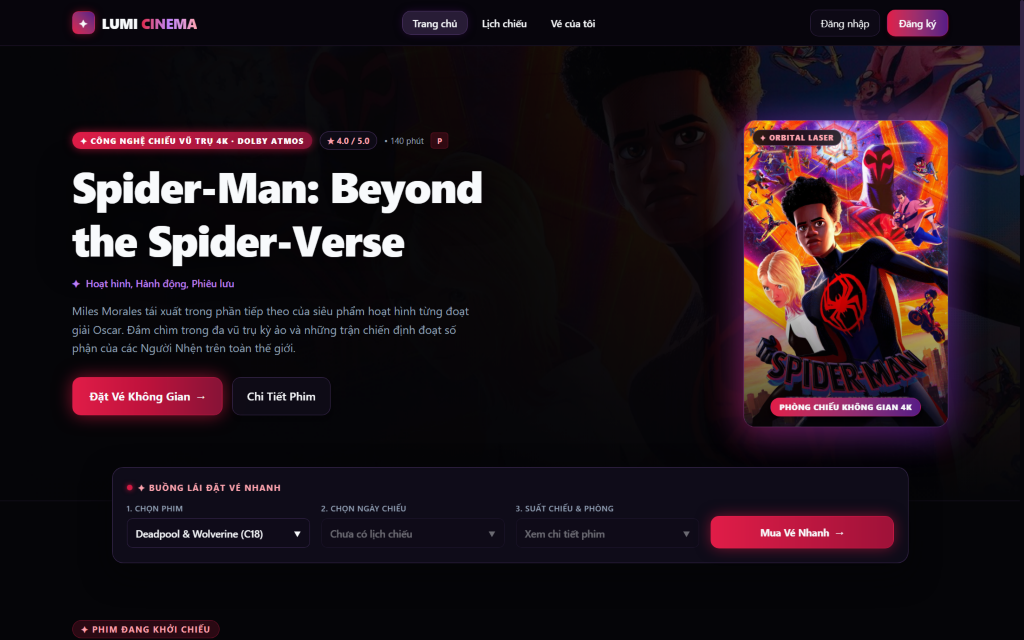
\includegraphics[width=\textwidth,height=0.55\textheight,keepaspectratio]{images/ui/3.4_trang_chu.png}
  \caption{Giao diện Trang chủ LumiCinema (/)}
  \label{fig:ui_3_4}
\end{figure}
\begin{itemize}[leftmargin=1.2cm]
  \item \textbf{Danh sách thành phần:} Thanh điều hướng (Logo, Phim, Vé của tôi, Đăng nhập/Đăng ký), Banner phim nổi bật, Thanh tìm kiếm \& lọc thể loại/trạng thái phim, Lưới thẻ phim (Poster, tên phim, thời lượng, đánh giá sao, nút Đặt vé).
  \item \textbf{Danh sách biến cố:} Nhấn chọn phim $\rightarrow$ chuyển trang Chi tiết phim; Nhập từ khóa/chọn bộ lọc $\rightarrow$ lọc danh sách phim theo thời gian thực; Nhấn Đăng nhập/Đăng ký $\rightarrow$ mở trang xác thực.
\end{itemize}

\subsection{Giao diện Đăng nhập}
\begin{figure}[H]
  \centering
  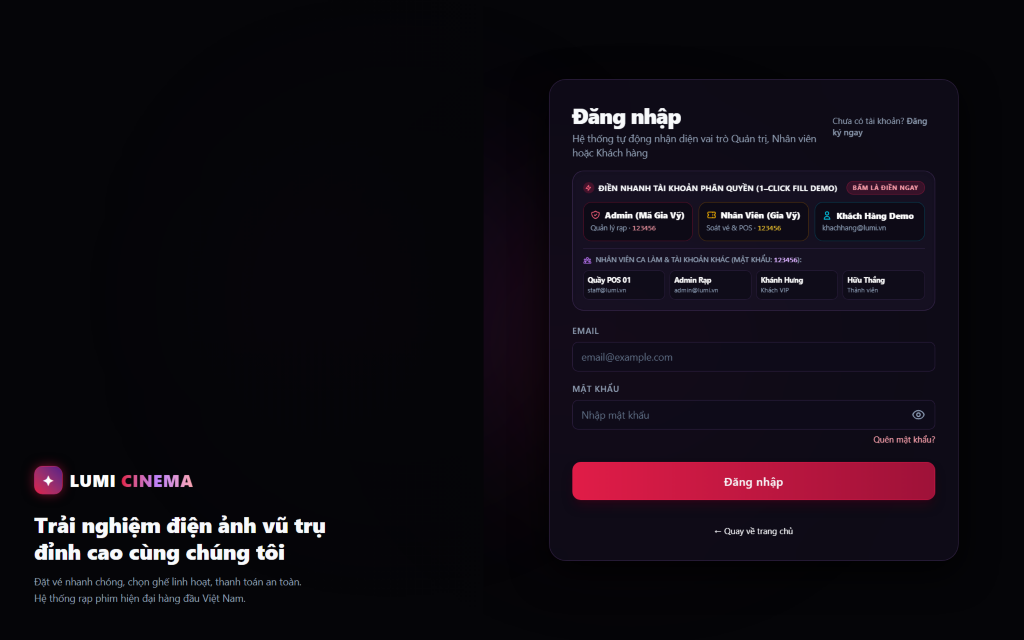
\includegraphics[width=\textwidth,height=0.55\textheight,keepaspectratio]{images/ui/3.5_dang_nhap.png}
  \caption{Giao diện Đăng nhập (/login)}
  \label{fig:ui_3_5}
\end{figure}
\begin{itemize}[leftmargin=1.2cm]
  \item \textbf{Danh sách thành phần:} Ô nhập Email, Ô nhập Mật khẩu, Nút Đăng nhập, Liên kết chuyển sang trang Đăng ký, Vùng hiển thị thông báo lỗi.
  \item \textbf{Danh sách biến cố:} Nhấn ``Đăng nhập'' $\rightarrow$ gọi \texttt{POST /api/auth/callback/credentials}, xác thực mật khẩu, lưu phiên làm việc (JWT Cookie) và điều hướng theo vai trò (Khách hàng / Nhân viên / Admin).
\end{itemize}

\subsection{Giao diện Đăng ký tài khoản}
\begin{figure}[H]
  \centering
  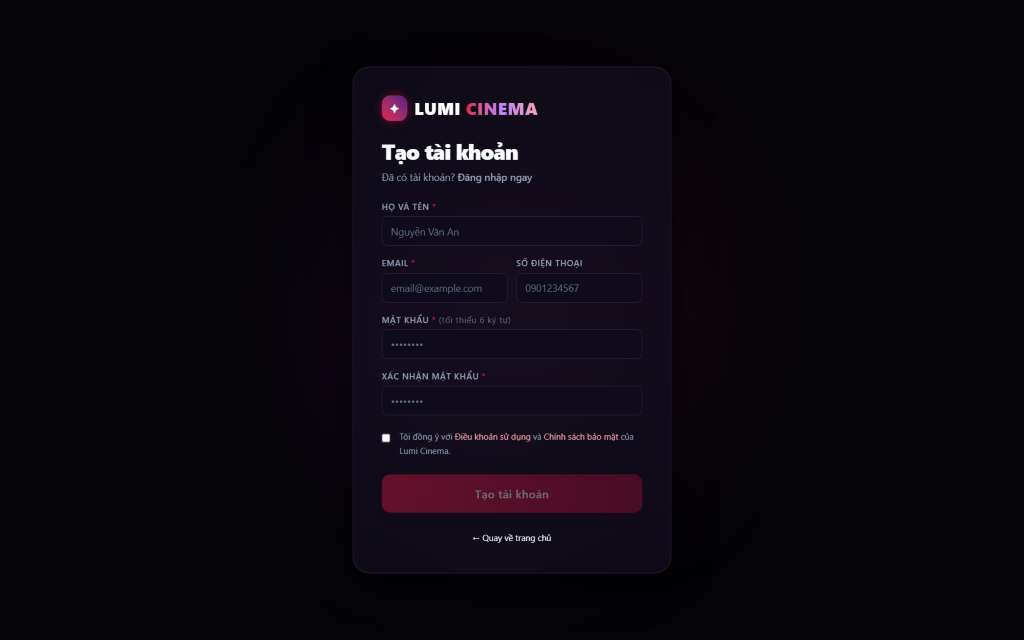
\includegraphics[width=\textwidth,height=0.55\textheight,keepaspectratio]{images/ui/3.6_dang_ky.png}
  \caption{Giao diện Đăng ký tài khoản (/signup)}
  \label{fig:ui_3_6}
\end{figure}
\begin{itemize}[leftmargin=1.2cm]
  \item \textbf{Danh sách thành phần:} Ô nhập Họ tên, Email, Số điện thoại, Mật khẩu, Xác nhận mật khẩu, Nút Đăng ký.
  \item \textbf{Danh sách biến cố:} Nhấn ``Đăng ký'' $\rightarrow$ kiểm tra hợp lệ dữ liệu, gọi \texttt{POST /api/auth/signup}, mã hóa mật khẩu bằng bcrypt và tạo tài khoản khách hàng mới.
\end{itemize}

\subsection{Giao diện Chi tiết phim và Chọn suất chiếu}
\begin{figure}[H]
  \centering
  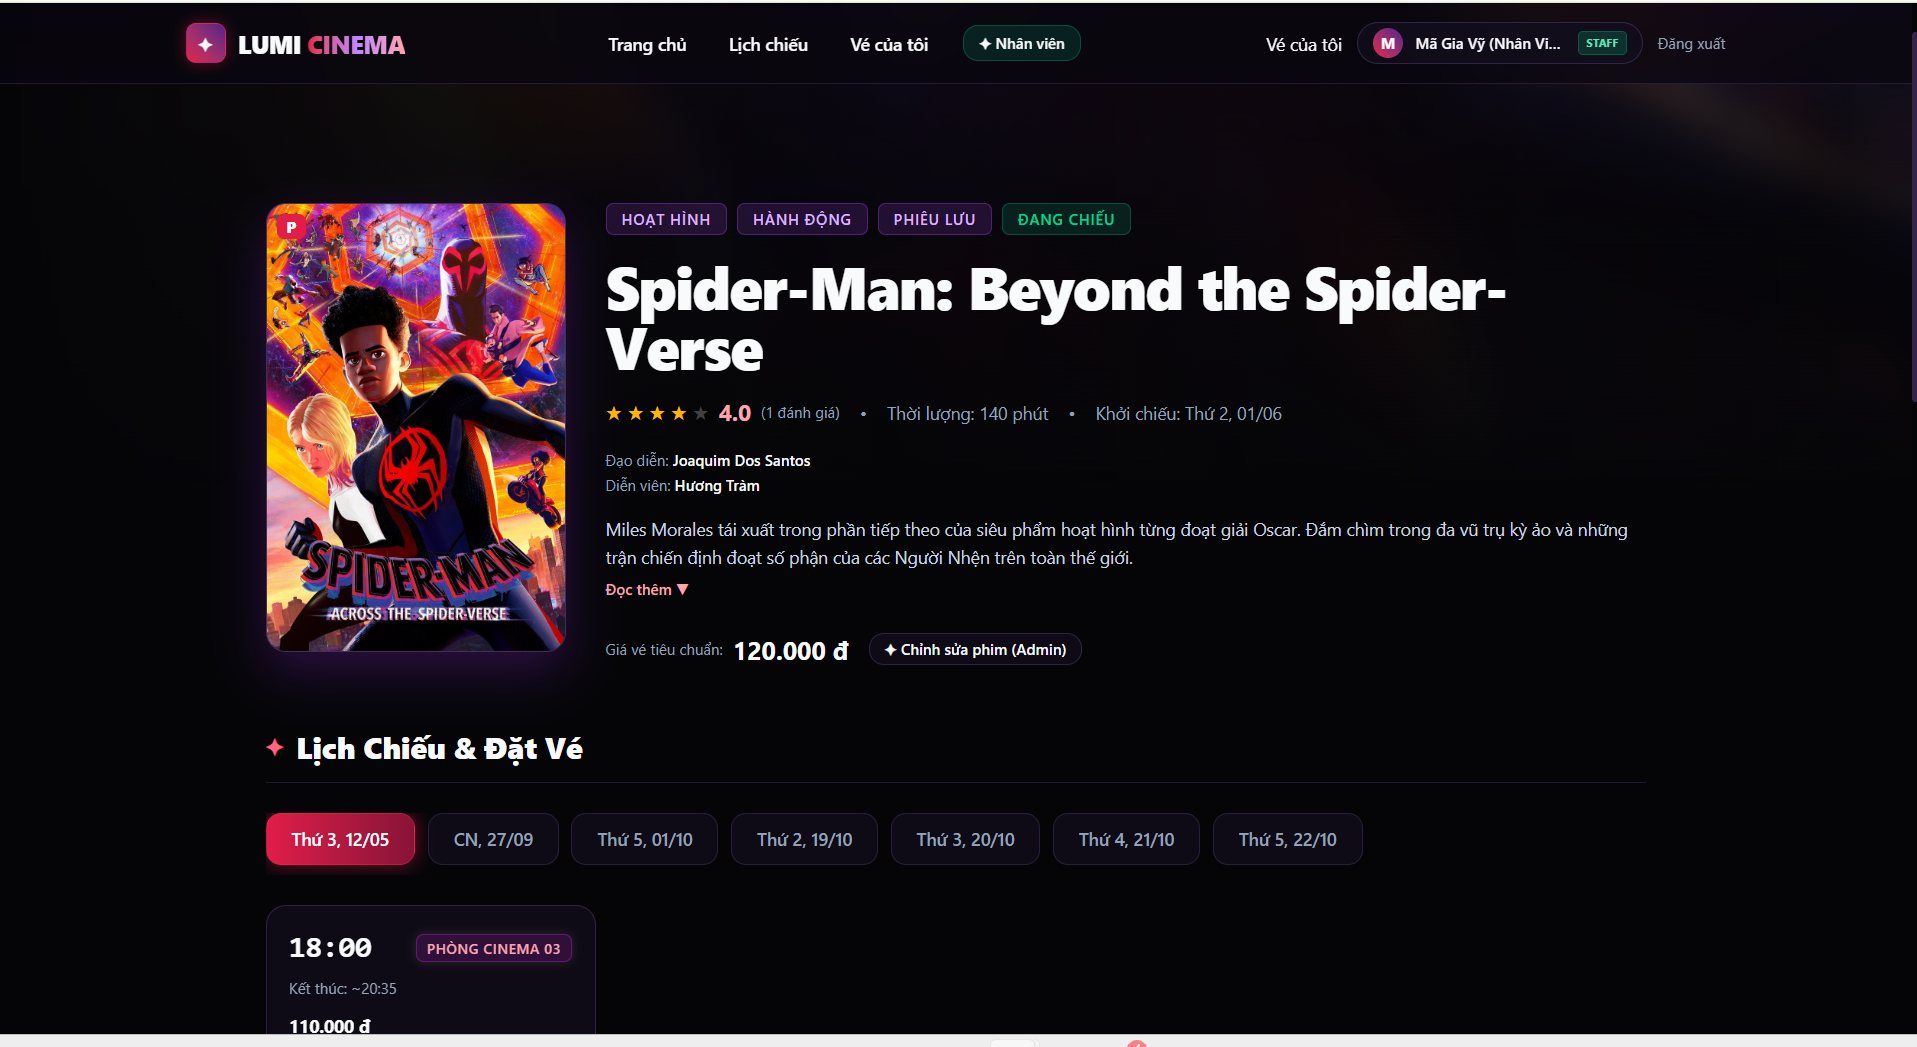
\includegraphics[width=\textwidth,height=0.55\textheight,keepaspectratio]{images/ui/3.7_chi_tiet_phim.png}
  \caption{Giao diện Chi tiết phim \& Lịch suất chiếu (/movies/[id])}
  \label{fig:ui_3_7}
\end{figure}
\begin{itemize}[leftmargin=1.2cm]
  \item \textbf{Danh sách thành phần:} Poster, Thông tin phim (thể loại, thời lượng, mô tả, điểm đánh giá trung bình), Bộ chọn ngày chiếu, Danh sách nút khung giờ suất chiếu, Khu vực đánh giá phim (1--5 sao và bình luận).
  \item \textbf{Danh sách biến cố:} Chọn ngày chiếu $\rightarrow$ cập nhật danh sách suất chiếu; Nhấn khung giờ $\rightarrow$ chuyển sang màn hình Chọn ghế; Gửi đánh giá $\rightarrow$ gọi \texttt{POST /api/reviews}.
\end{itemize}

\subsection{Giao diện Chọn ghế và Giữ chỗ 10 phút}
\begin{figure}[H]
  \centering
  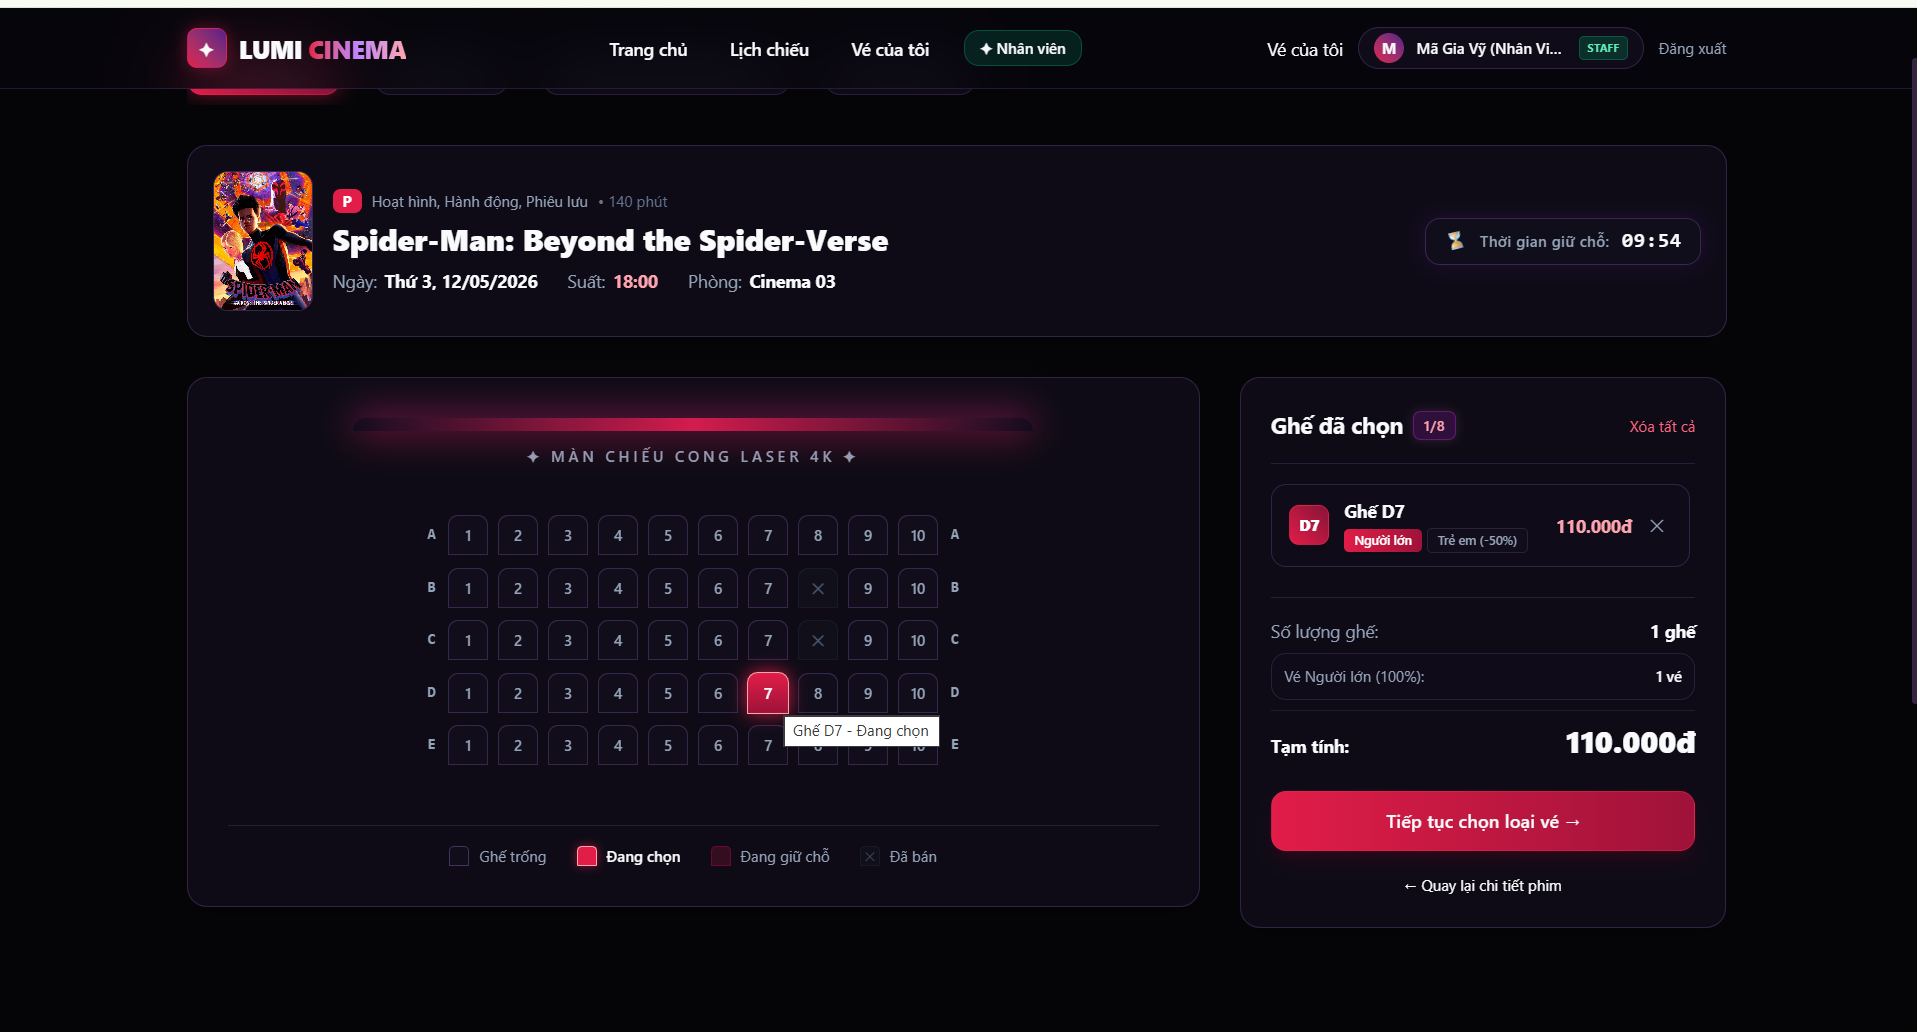
\includegraphics[width=\textwidth,height=0.55\textheight,keepaspectratio]{images/ui/3.8_chon_ghe.png}
  \caption{Giao diện Chọn ghế phòng chiếu A1--E10 (/screenings/[id]/seats)}
  \label{fig:ui_3_8}
\end{figure}
\begin{itemize}[leftmargin=1.2cm]
  \item \textbf{Danh sách thành phần:} Thanh màn hình chiếu, Lưới 50 nút ghế A1--E10 (Trống / Đang chọn / Đang giữ / Đã đặt), Bộ chọn loại vé (Thường / Trẻ em), Bảng tóm tắt ghế đã chọn \& tạm tính, Nút Tiếp tục.
  \item \textbf{Danh sách biến cố:} Nhấn chọn/bỏ chọn ghế (tối đa 8 ghế) $\rightarrow$ cập nhật danh sách ghế và tổng tiền; Nhấn ``Tiếp tục'' $\rightarrow$ gọi \texttt{POST /api/seats/reserve} giữ ghế 10 phút và chuyển sang bước Chọn Combo.
\end{itemize}

\subsection{Giao diện Chọn Combo bắp nước}
\begin{figure}[H]
  \centering
  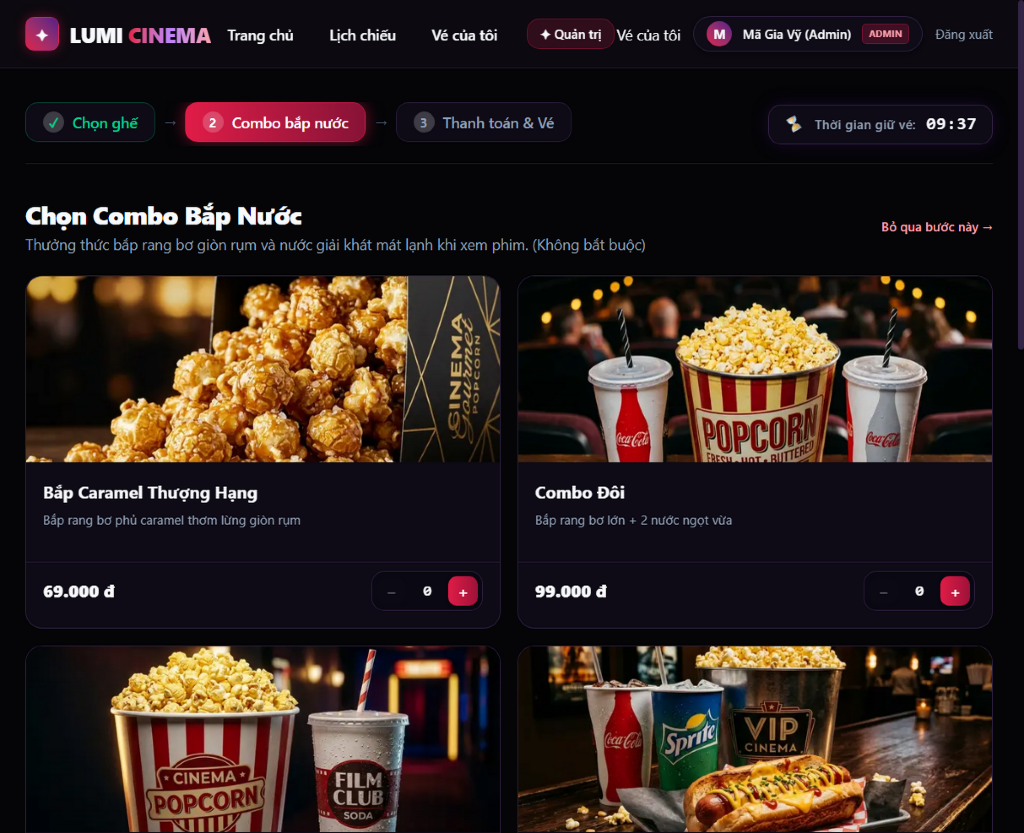
\includegraphics[width=\textwidth,height=0.55\textheight,keepaspectratio]{images/ui/3.9_chon_combo.png}
  \caption{Giao diện Chọn Combo bắp nước (/screenings/[id]/checkout/combo)}
  \label{fig:ui_3_9}
\end{figure}
\begin{itemize}[leftmargin=1.2cm]
  \item \textbf{Danh sách thành phần:} Đồng hồ đếm ngược 10 phút giữ chỗ, Danh sách thẻ Combo (hình ảnh, giá, tồn kho, nút tăng/giảm số lượng), Nút Bỏ qua / Tiếp tục thanh toán.
  \item \textbf{Danh sách biến cố:} Tăng/giảm combo $\rightarrow$ cập nhật tổng tiền; Nhấn Tiếp tục $\rightarrow$ giữ tồn kho combo 10 phút và chuyển sang màn hình Checkout.
\end{itemize}

\subsection{Giao diện Thanh toán đơn đặt vé (Checkout)}
\begin{figure}[H]
  \centering
  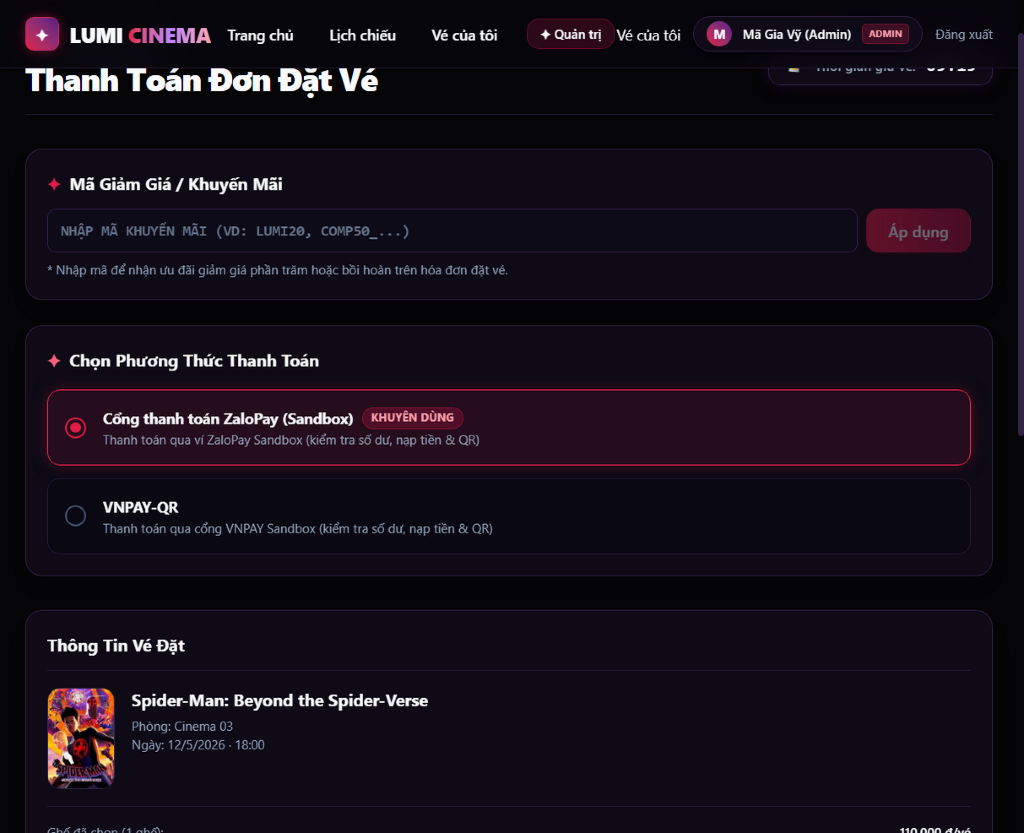
\includegraphics[width=\textwidth,height=0.55\textheight,keepaspectratio]{images/ui/3.10_checkout.png}
  \caption{Giao diện Thanh toán Checkout (/screenings/[id]/checkout)}
  \label{fig:ui_3_10}
\end{figure}
\begin{itemize}[leftmargin=1.2cm]
  \item \textbf{Danh sách thành phần:} Tóm tắt vé và combo, Ô nhập mã Voucher \& nút Áp dụng, Bộ chọn cổng thanh toán (ZaloPay / VNPay), Nút Thanh toán.
  \item \textbf{Danh sách biến cố:} Áp dụng voucher $\rightarrow$ gọi \texttt{POST /api/coupons/validate}; Nhấn Thanh toán $\rightarrow$ gọi \texttt{POST /api/payments/initiate} và chuyển hướng sang cổng thanh toán.
\end{itemize}

\subsection{Giao diện Cổng thanh toán ZaloPay Gateway}
\begin{figure}[H]
  \centering
  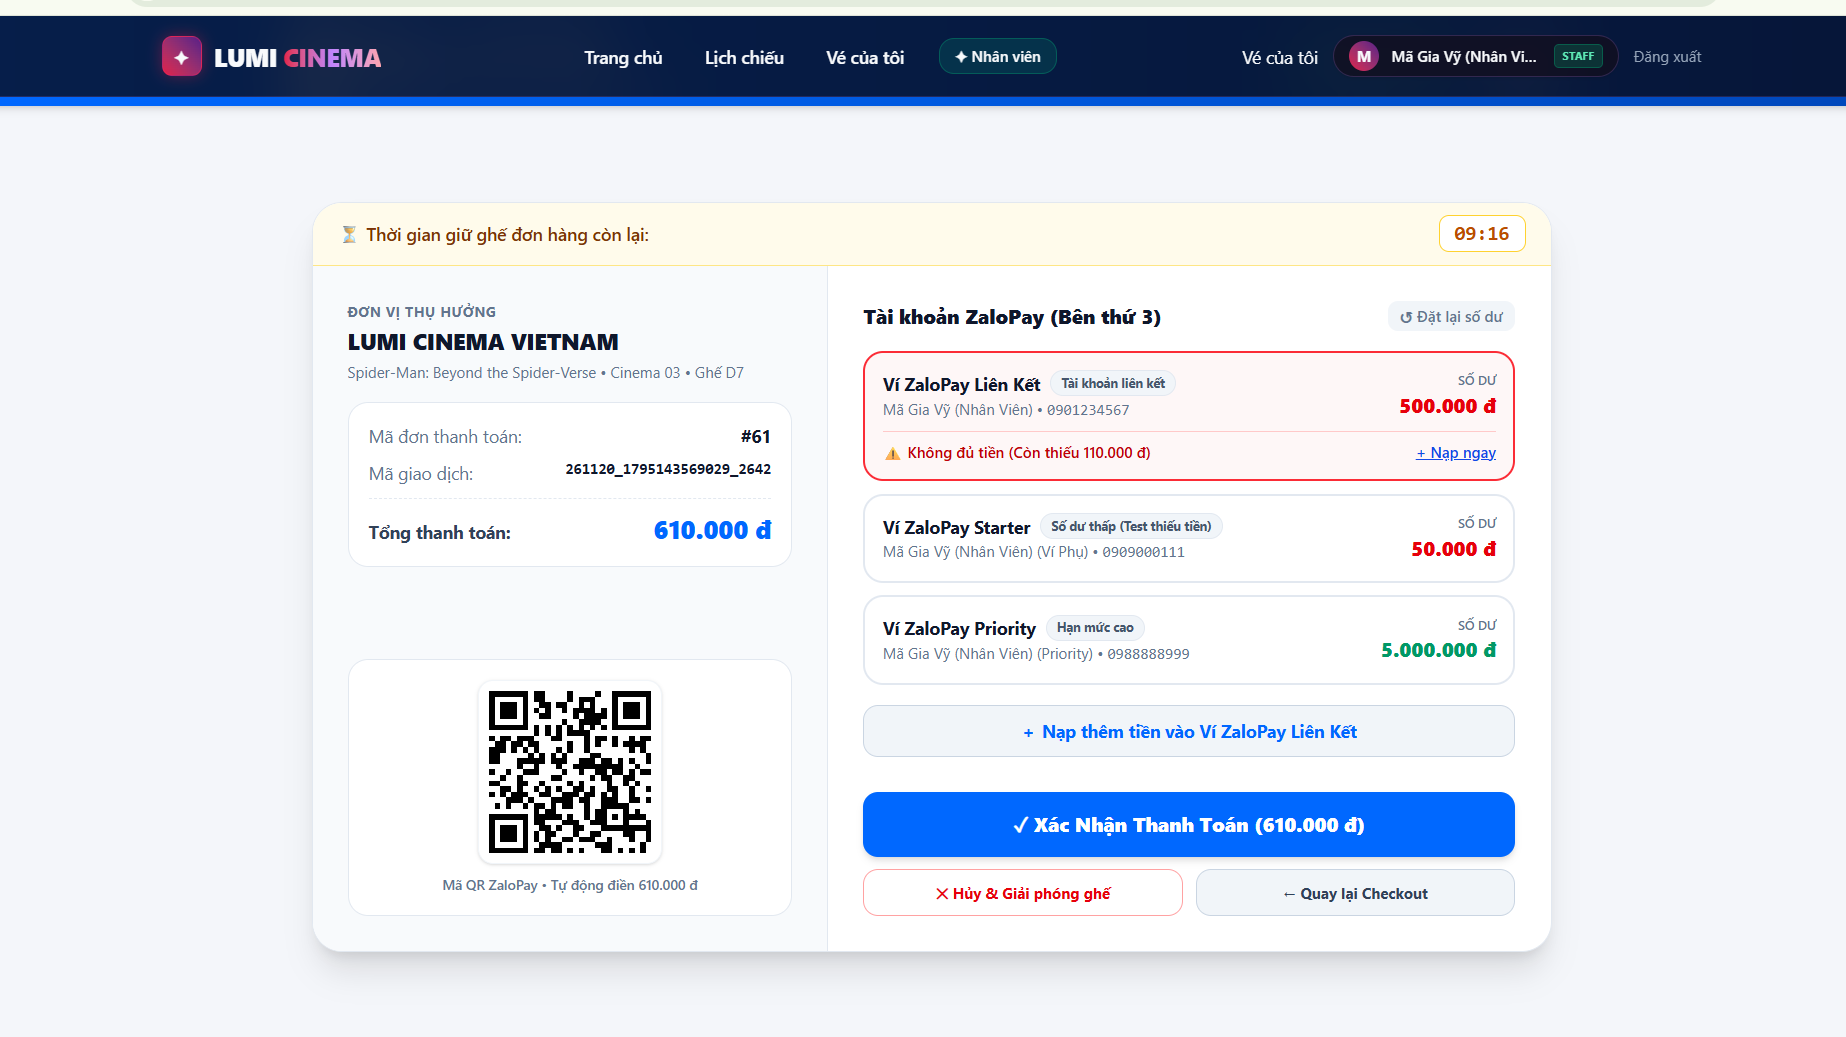
\includegraphics[width=\textwidth,height=0.55\textheight,keepaspectratio]{images/ui/3.11_zalopay_gateway.png}
  \caption{Giao diện Cổng thanh toán nội bộ ZaloPay (/payments/zalopay-mock)}
  \label{fig:ui_3_11}
\end{figure}

\subsection{Giao diện Cổng thanh toán VNPay Gateway}
\begin{figure}[H]
  \centering
  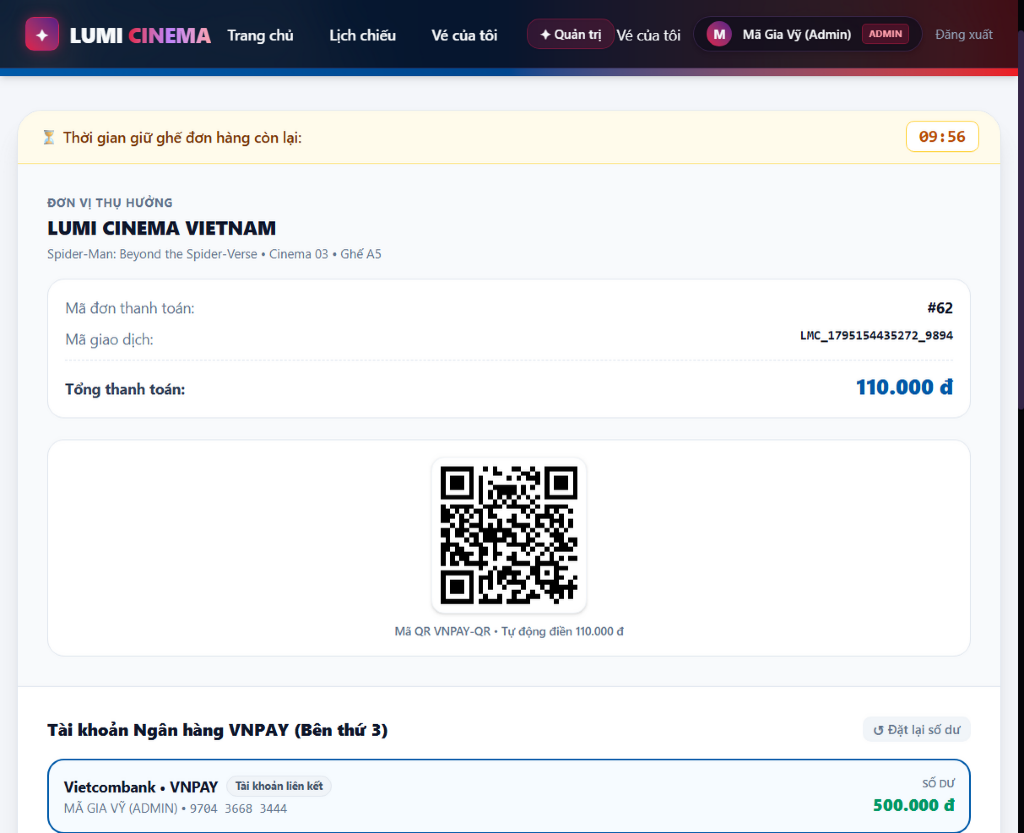
\includegraphics[width=\textwidth,height=0.55\textheight,keepaspectratio]{images/ui/3.12_vnpay_gateway.png}
  \caption{Giao diện Cổng thanh toán nội bộ VNPAY-QR (/payments/vnpay-mock)}
  \label{fig:ui_3_12}
\end{figure}

\subsection{Giao diện Vé của tôi (Quản lý vé khách hàng)}
\begin{figure}[H]
  \centering
  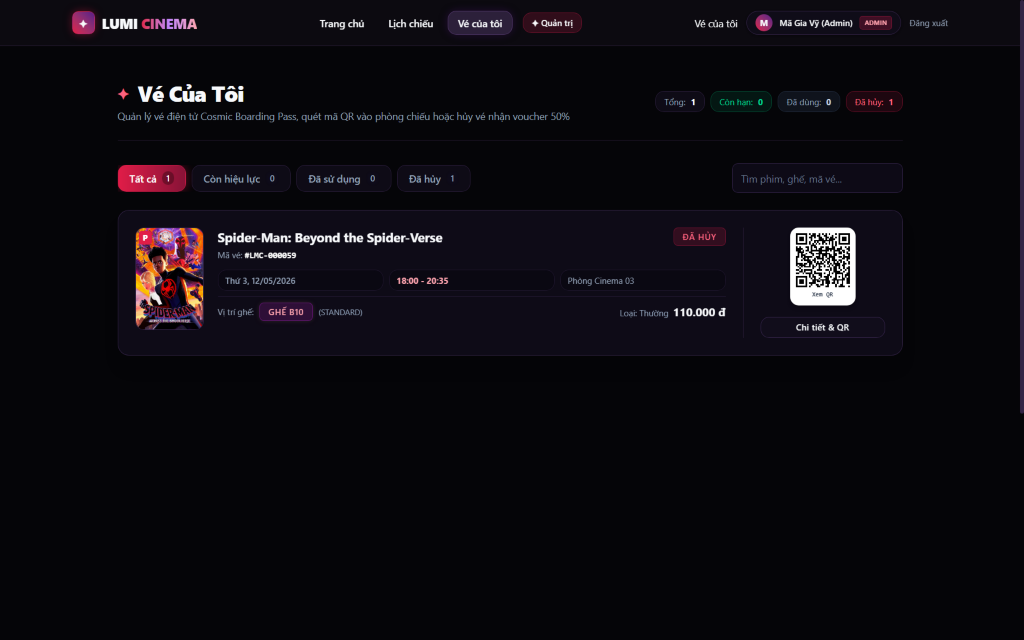
\includegraphics[width=\textwidth,height=0.55\textheight,keepaspectratio]{images/ui/3.13_ve_cua_toi.png}
  \caption{Giao diện Quản lý Vé Của Tôi (/tickets)}
  \label{fig:ui_3_13}
\end{figure}

\subsection{Giao diện Bàn điều hành Nhân viên quầy}
\begin{figure}[H]
  \centering
  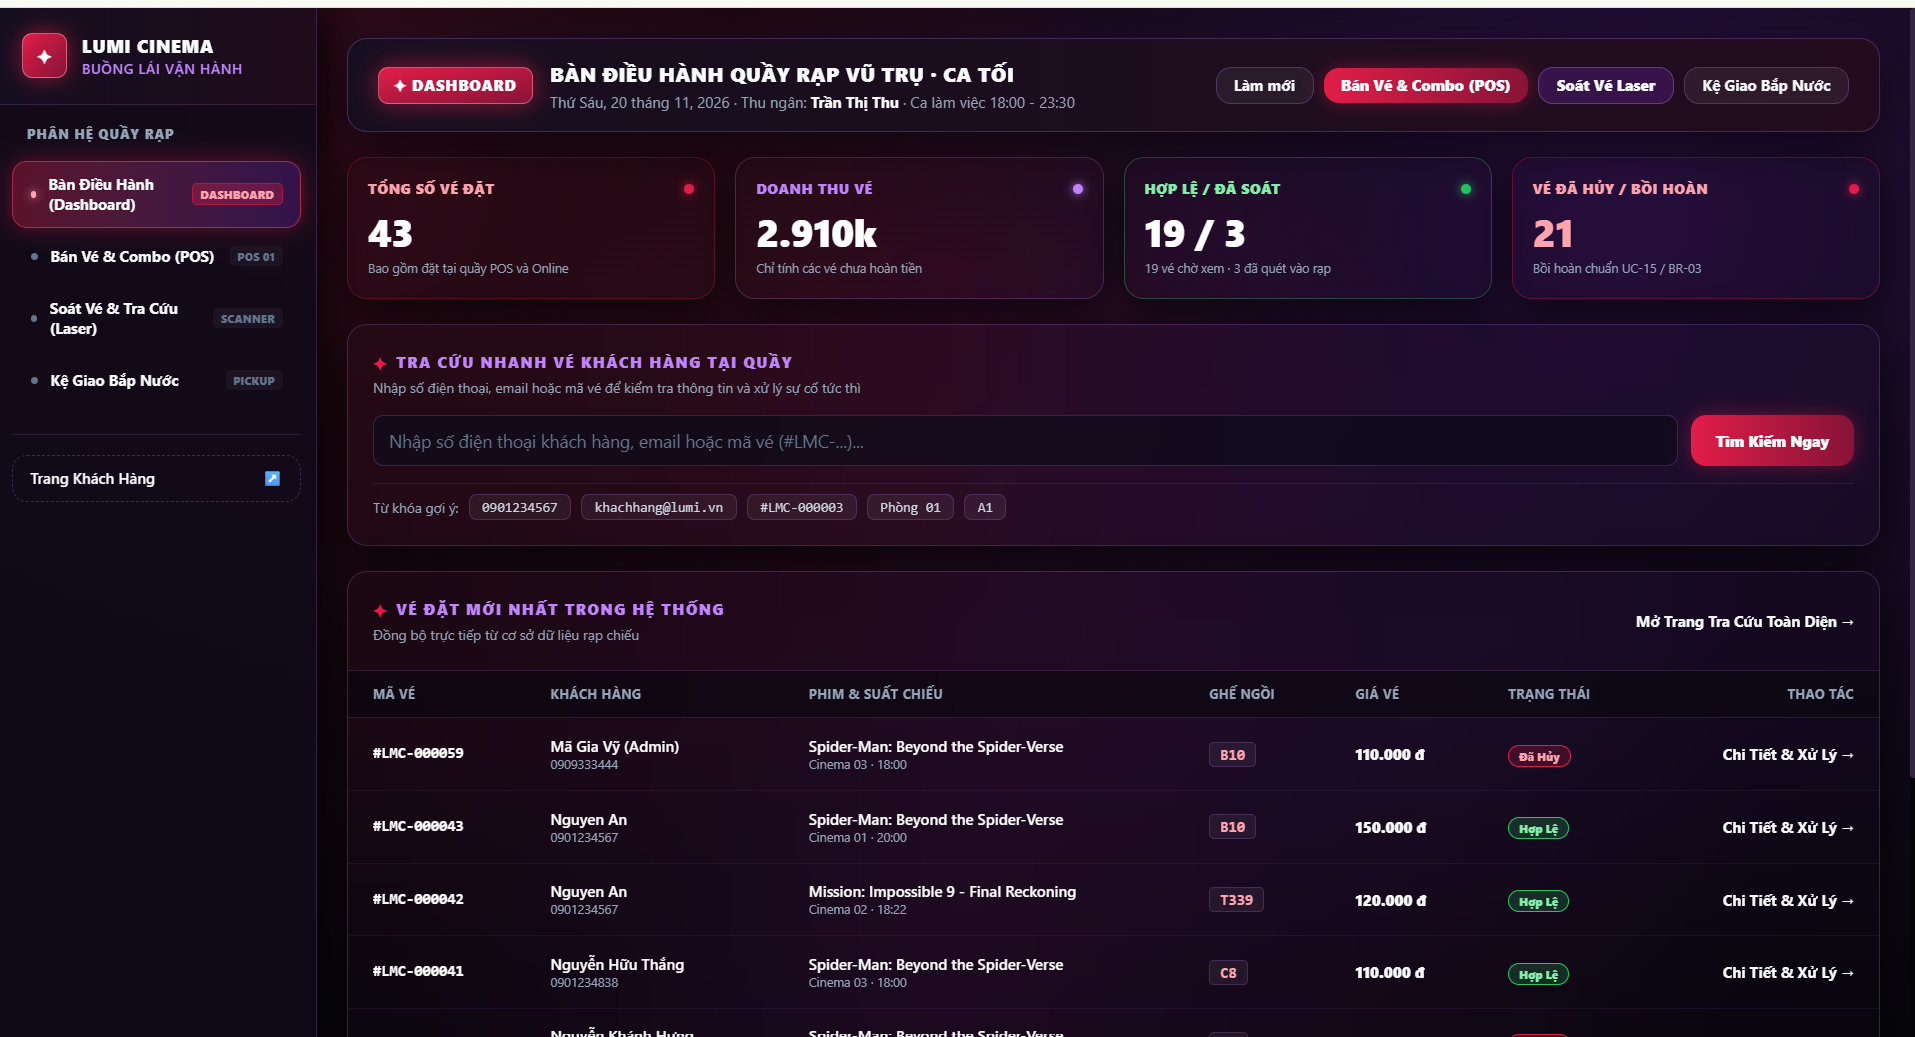
\includegraphics[width=\textwidth,height=0.55\textheight,keepaspectratio]{images/ui/3.14_staff_ban_dieu_hanh.png}
  \caption{Giao diện Bàn điều hành Quầy rạp (/staff)}
  \label{fig:ui_3_14}
\end{figure}

\subsection{Giao diện Bán vé và Combo tại quầy (POS)}
\begin{figure}[H]
  \centering
  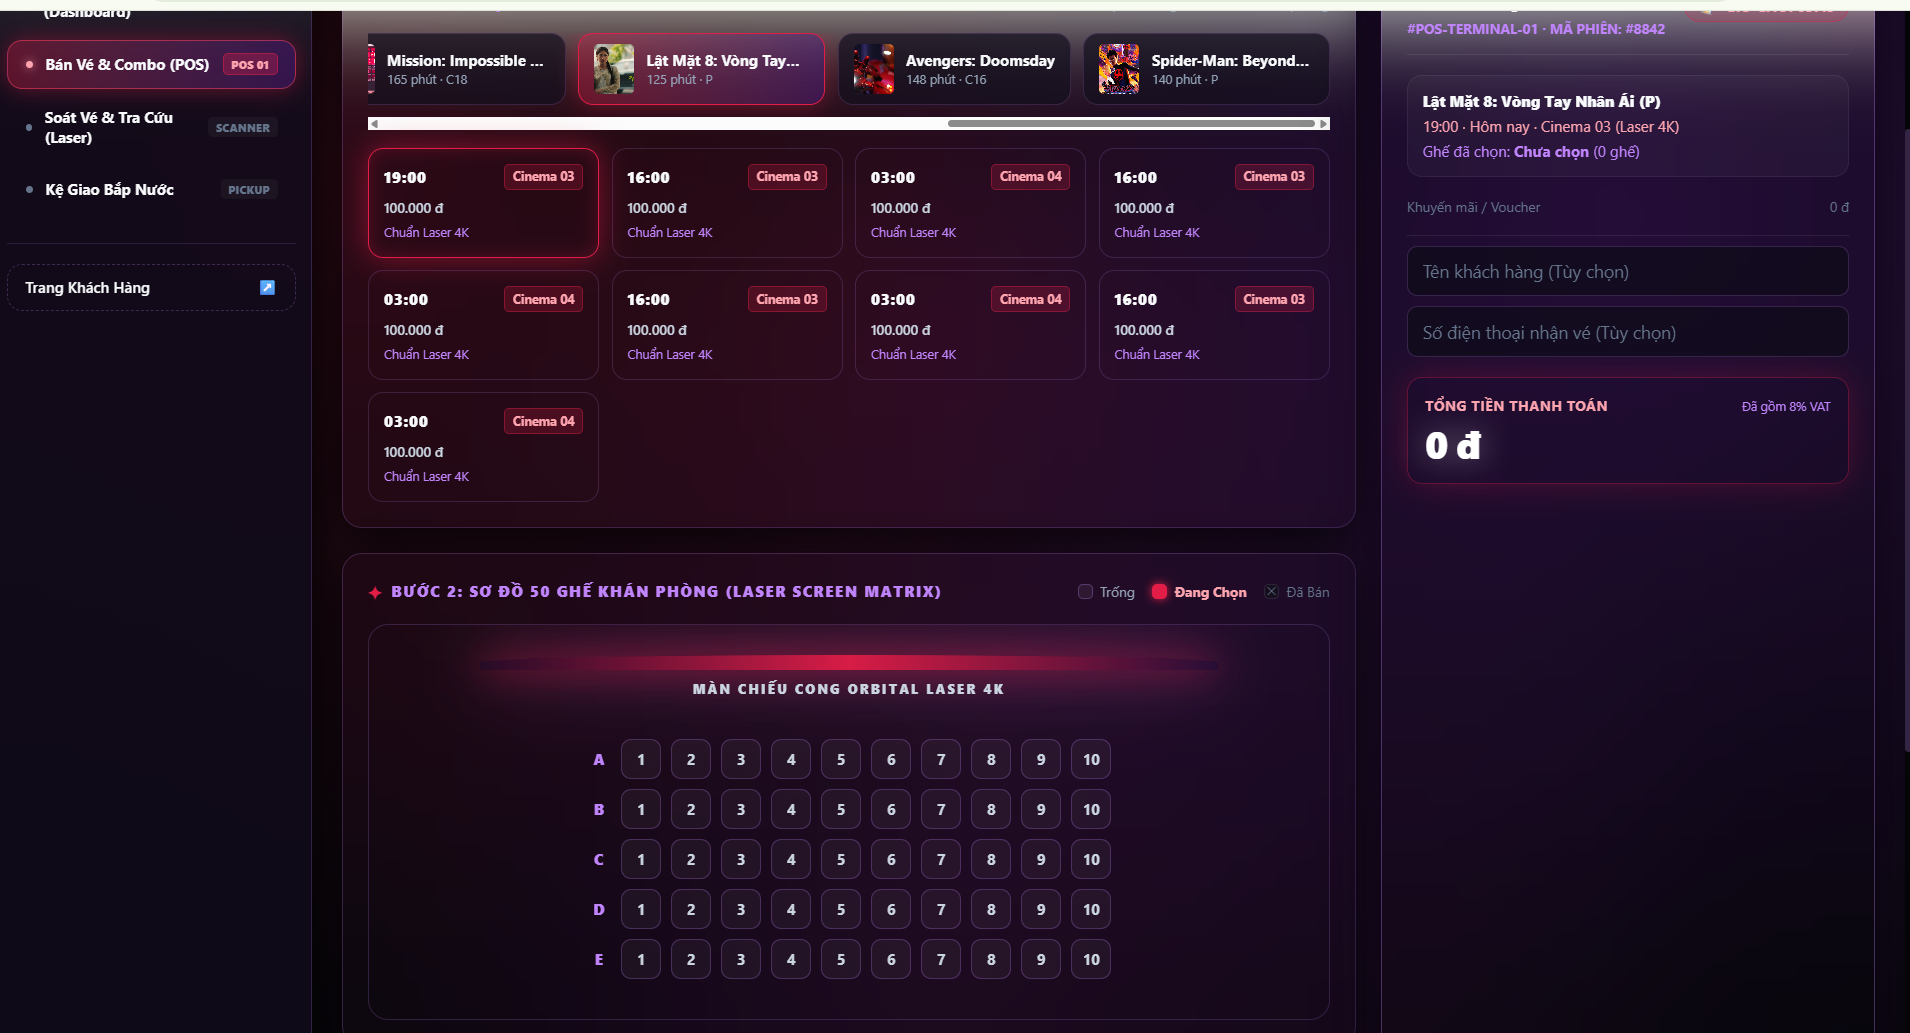
\includegraphics[width=\textwidth,height=0.55\textheight,keepaspectratio]{images/ui/3.15_staff_pos.png}
  \caption{Giao diện Bán vé \& Combo tại quầy POS (/staff/pos)}
  \label{fig:ui_3_15}
\end{figure}

\subsection{Giao diện Trạm Soát vé Laser \& Xử lý sự cố}
\begin{figure}[H]
  \centering
  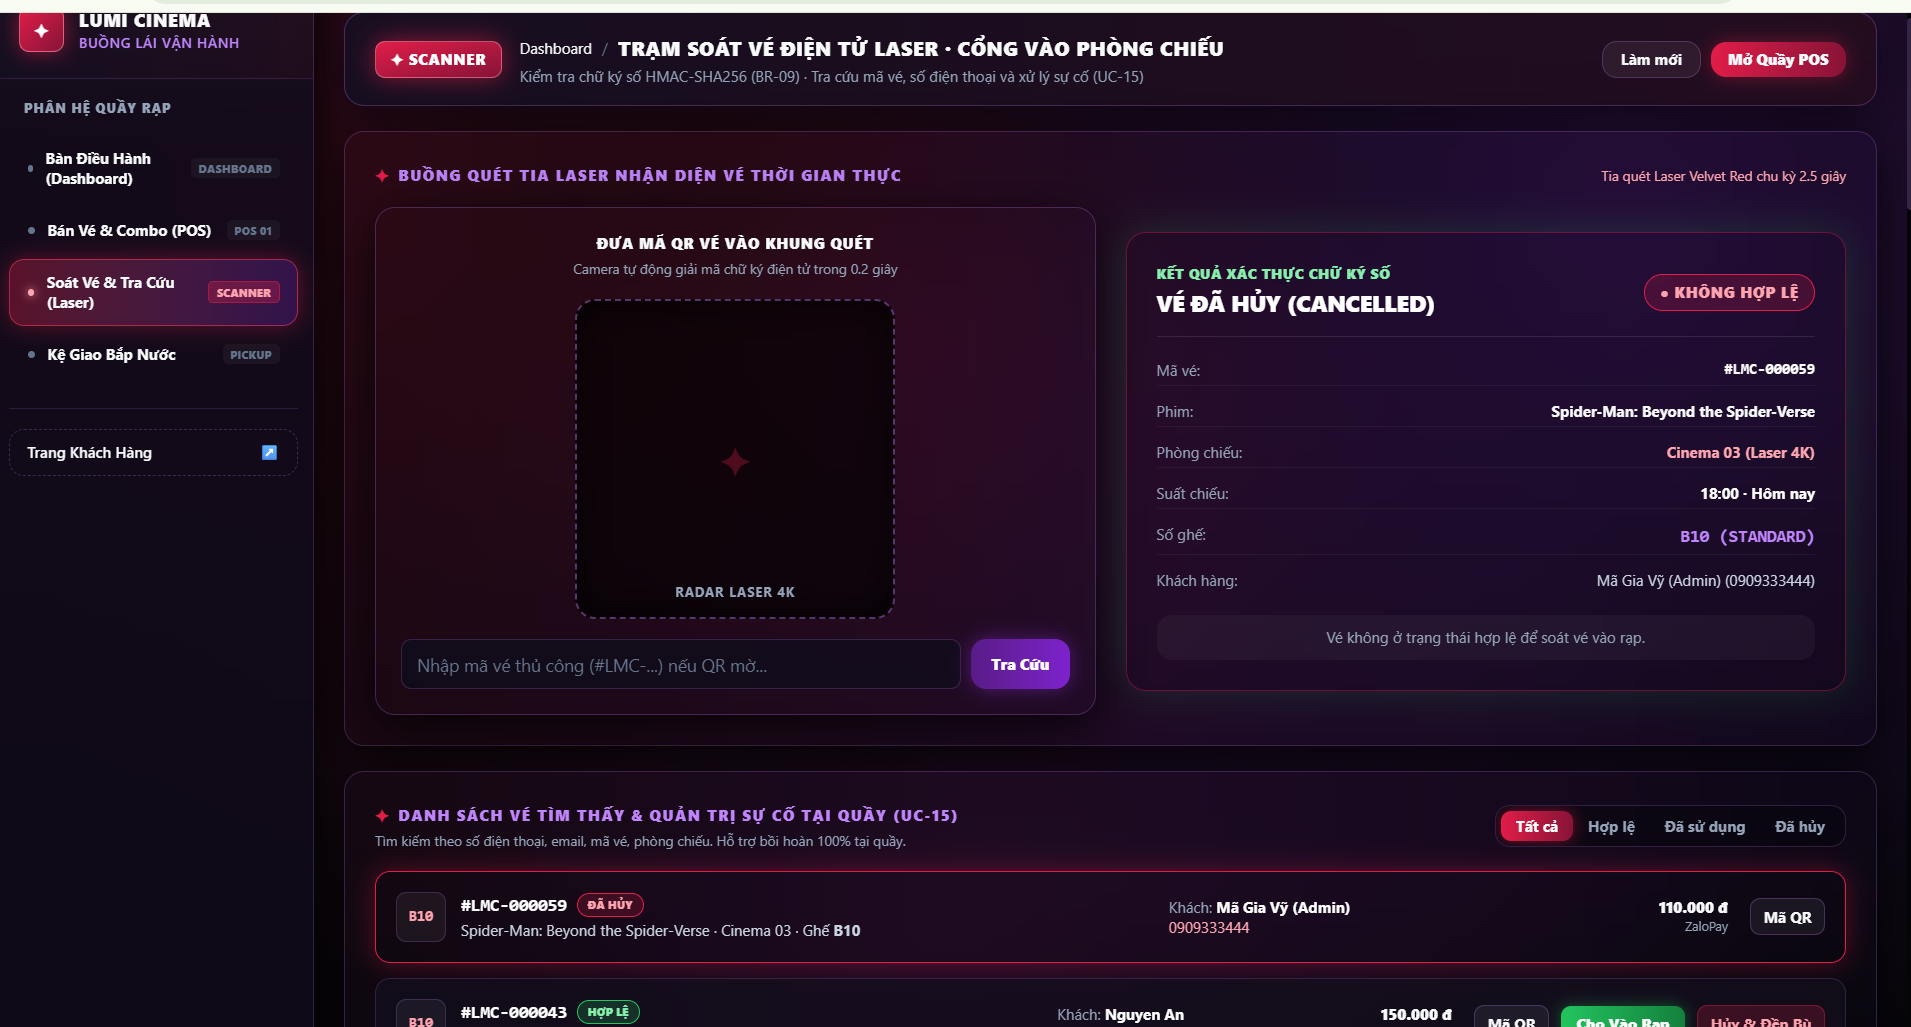
\includegraphics[width=\textwidth,height=0.55\textheight,keepaspectratio]{images/ui/3.16_staff_soat_ve.png}
  \caption{Giao diện Soát vé điện tử Laser \& Xử lý sự cố (/staff)}
  \label{fig:ui_3_16}
\end{figure}

\subsection{Giao diện Kệ giao Bắp Nước (Concession Queue)}
\begin{figure}[H]
  \centering
  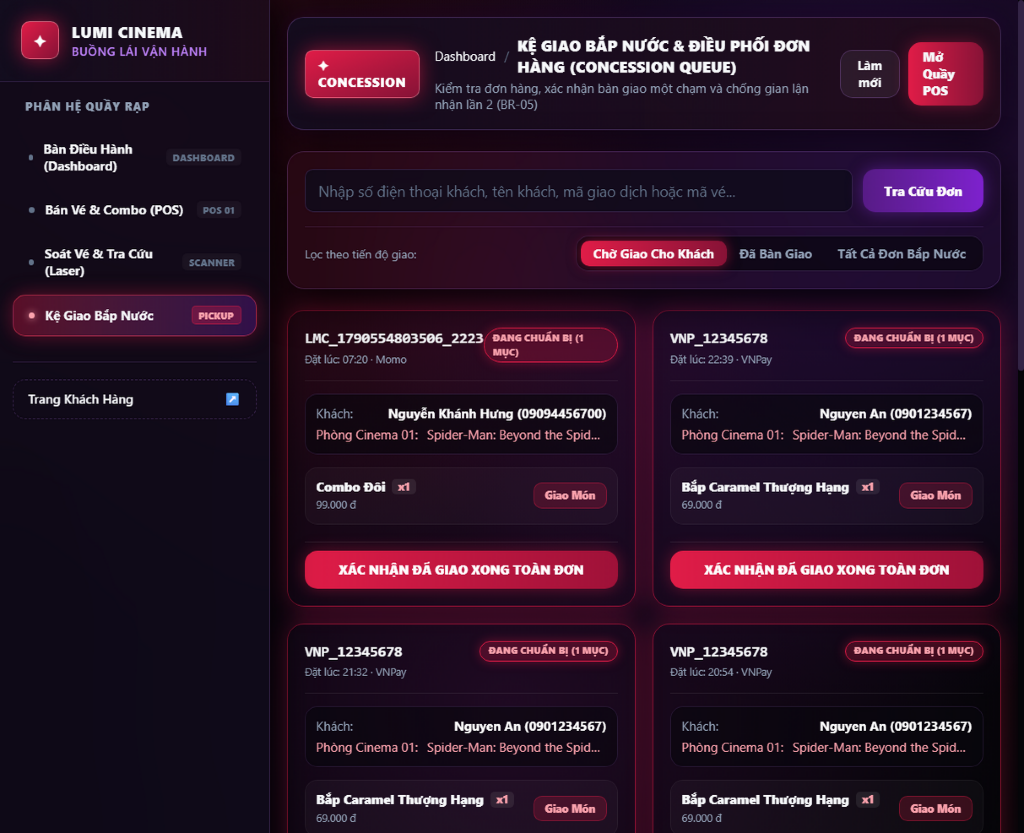
\includegraphics[width=\textwidth,height=0.55\textheight,keepaspectratio]{images/ui/3.17_staff_giao_combo.png}
  \caption{Giao diện Kệ Giao Bắp Nước tại quầy (/staff/combos)}
  \label{fig:ui_3_17}
\end{figure}

\subsection{Giao diện Admin Dashboard \& Giám sát 5 phòng chiếu}
\begin{figure}[H]
  \centering
  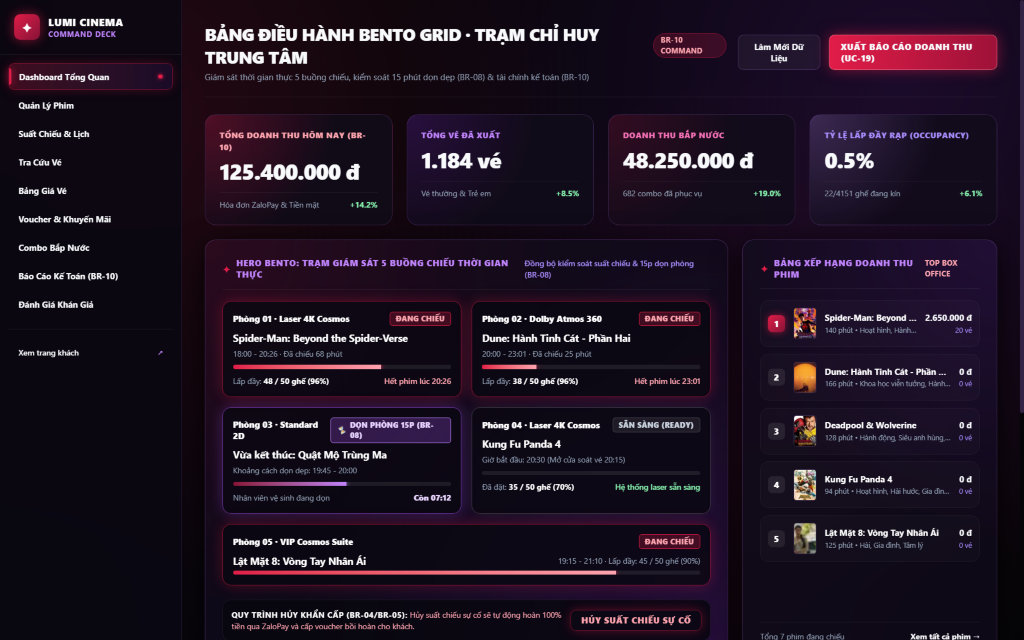
\includegraphics[width=\textwidth,height=0.55\textheight,keepaspectratio]{images/ui/3.18_admin_dashboard.png}
  \caption{Giao diện Admin Dashboard tổng quan (/admin/dashboard)}
  \label{fig:ui_3_18}
\end{figure}

\subsection{Giao diện Quản lý Danh mục Phim}
\begin{figure}[H]
  \centering
  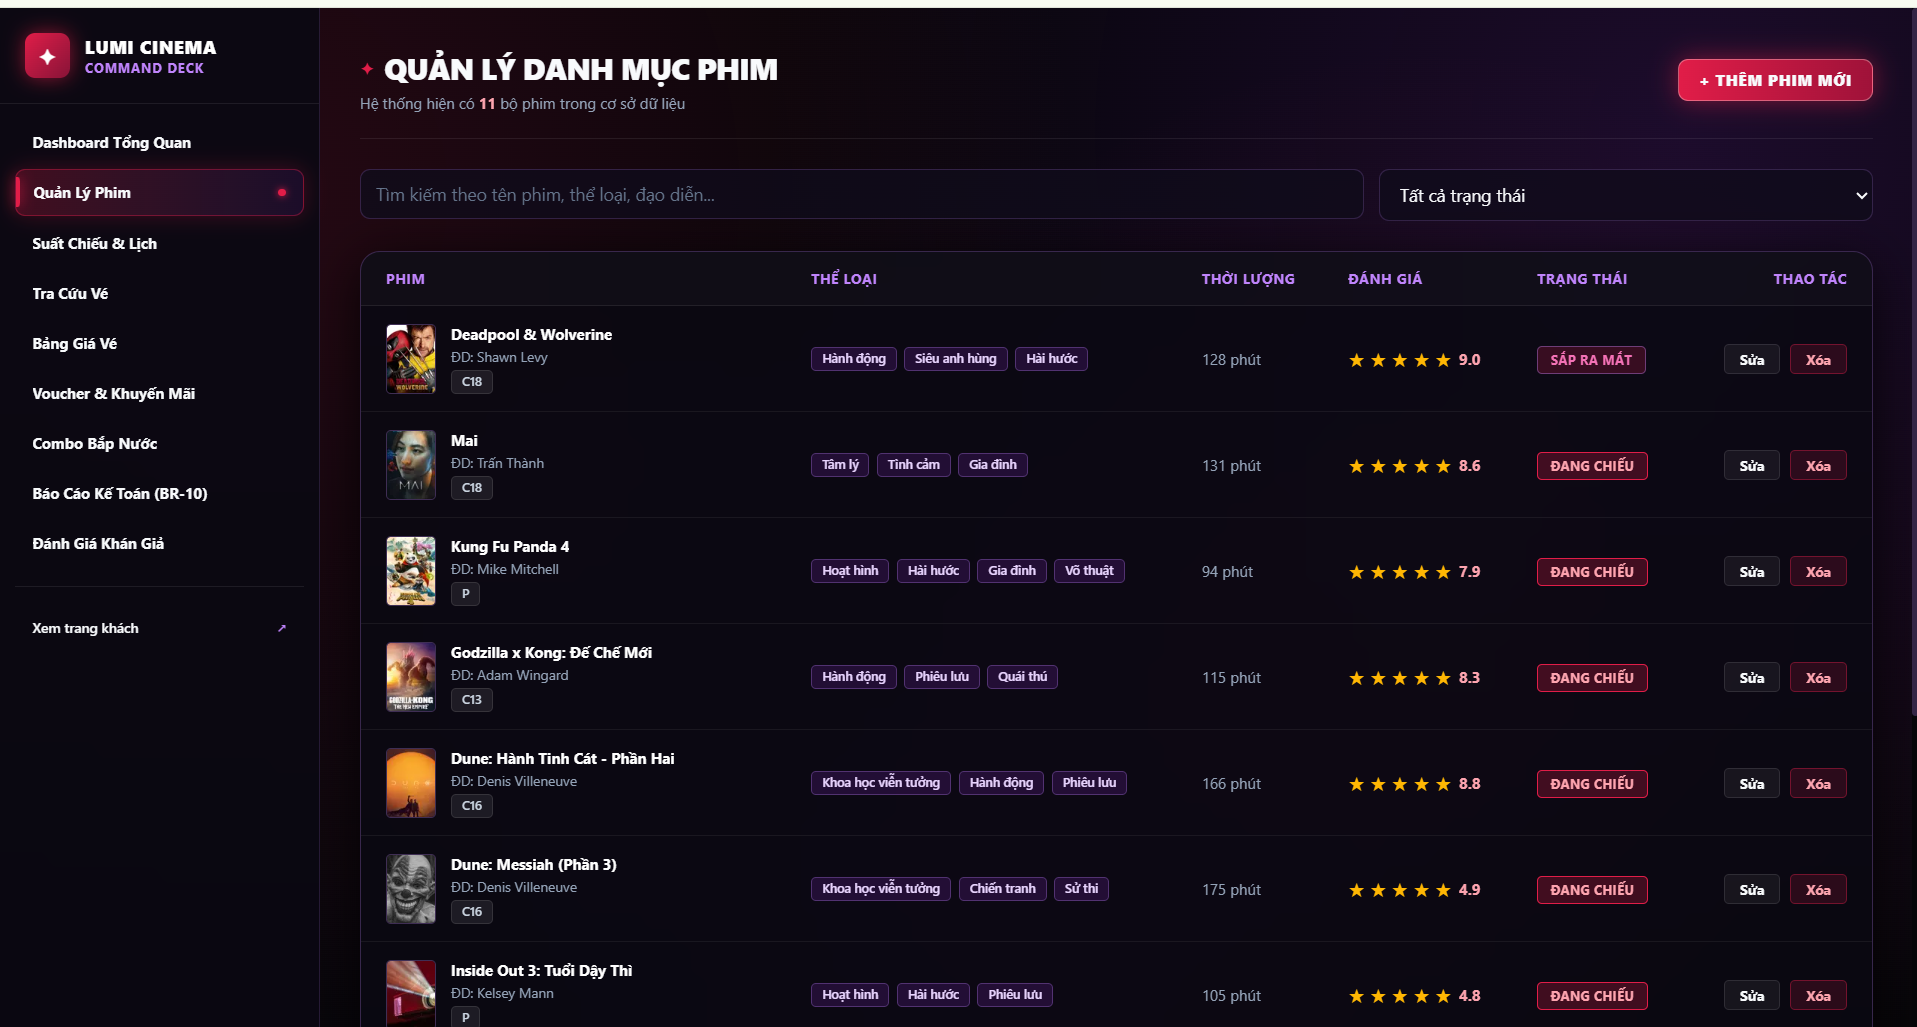
\includegraphics[width=\textwidth,height=0.55\textheight,keepaspectratio]{images/ui/3.19_admin_movies.png}
  \caption{Giao diện Quản lý Danh mục Phim (/admin/movies)}
  \label{fig:ui_3_19}
\end{figure}

\subsection{Giao diện Quản lý Suất chiếu \& Lịch chiếu}
\begin{figure}[H]
  \centering
  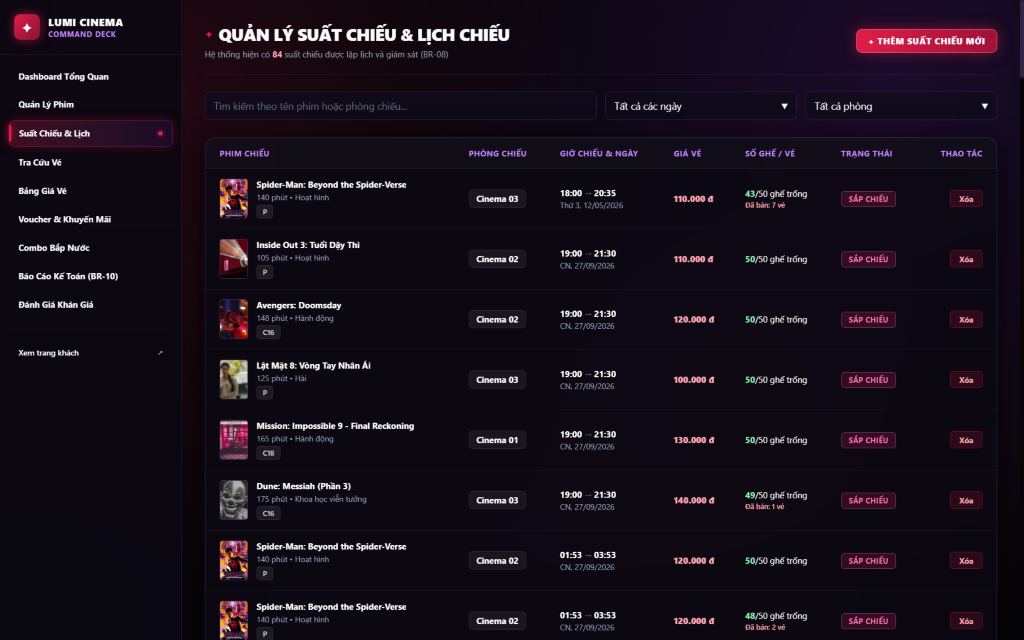
\includegraphics[width=\textwidth,height=0.55\textheight,keepaspectratio]{images/ui/3.20_admin_screenings.png}
  \caption{Giao diện Quản lý Suất chiếu \& Lịch chiếu (/admin/screenings)}
  \label{fig:ui_3_20}
\end{figure}

\subsection{Giao diện Quản lý Combo Bắp Nước}
\begin{figure}[H]
  \centering
  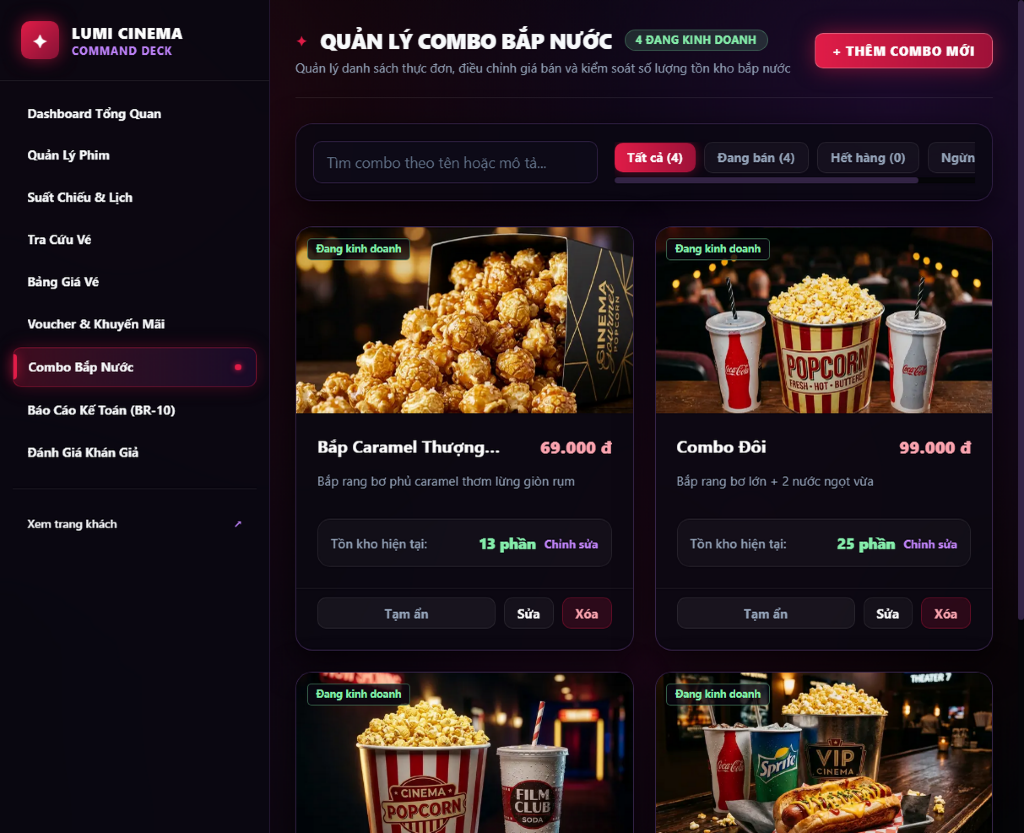
\includegraphics[width=\textwidth,height=0.55\textheight,keepaspectratio]{images/ui/3.21_admin_combos.png}
  \caption{Giao diện Quản lý Combo Bắp Nước (/admin/combos)}
  \label{fig:ui_3_21}
\end{figure}

\subsection{Giao diện Cấu hình Bảng giá vé hệ thống}
\begin{figure}[H]
  \centering
  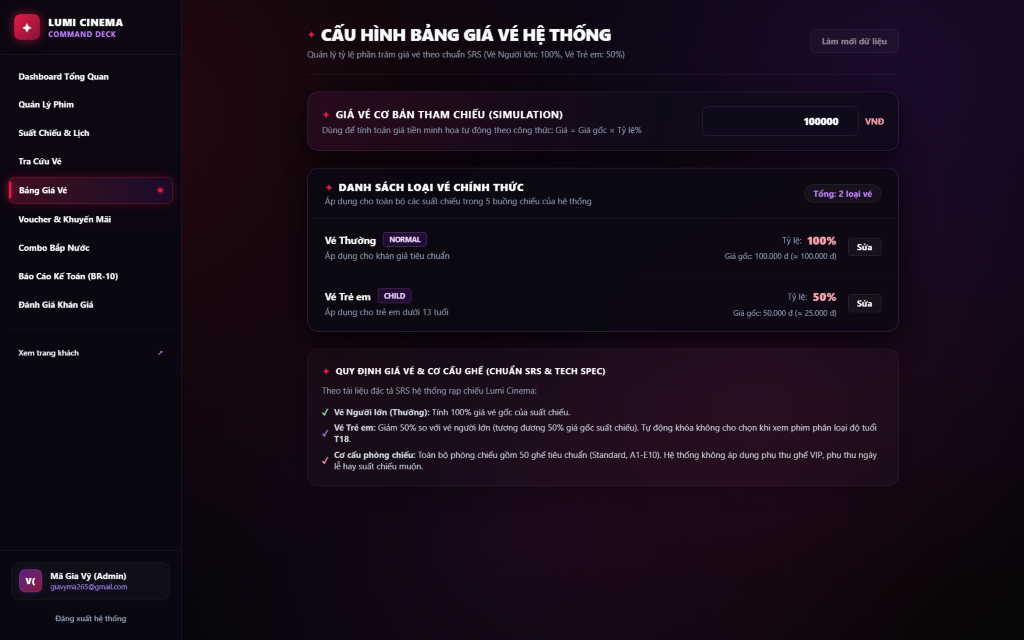
\includegraphics[width=\textwidth,height=0.55\textheight,keepaspectratio]{images/ui/3.22_admin_pricing.png}
  \caption{Giao diện Cấu hình Bảng Giá Vé (/admin/pricing)}
  \label{fig:ui_3_22}
\end{figure}

\subsection{Giao diện Quản lý Mã giảm giá \& Voucher}
\begin{figure}[H]
  \centering
  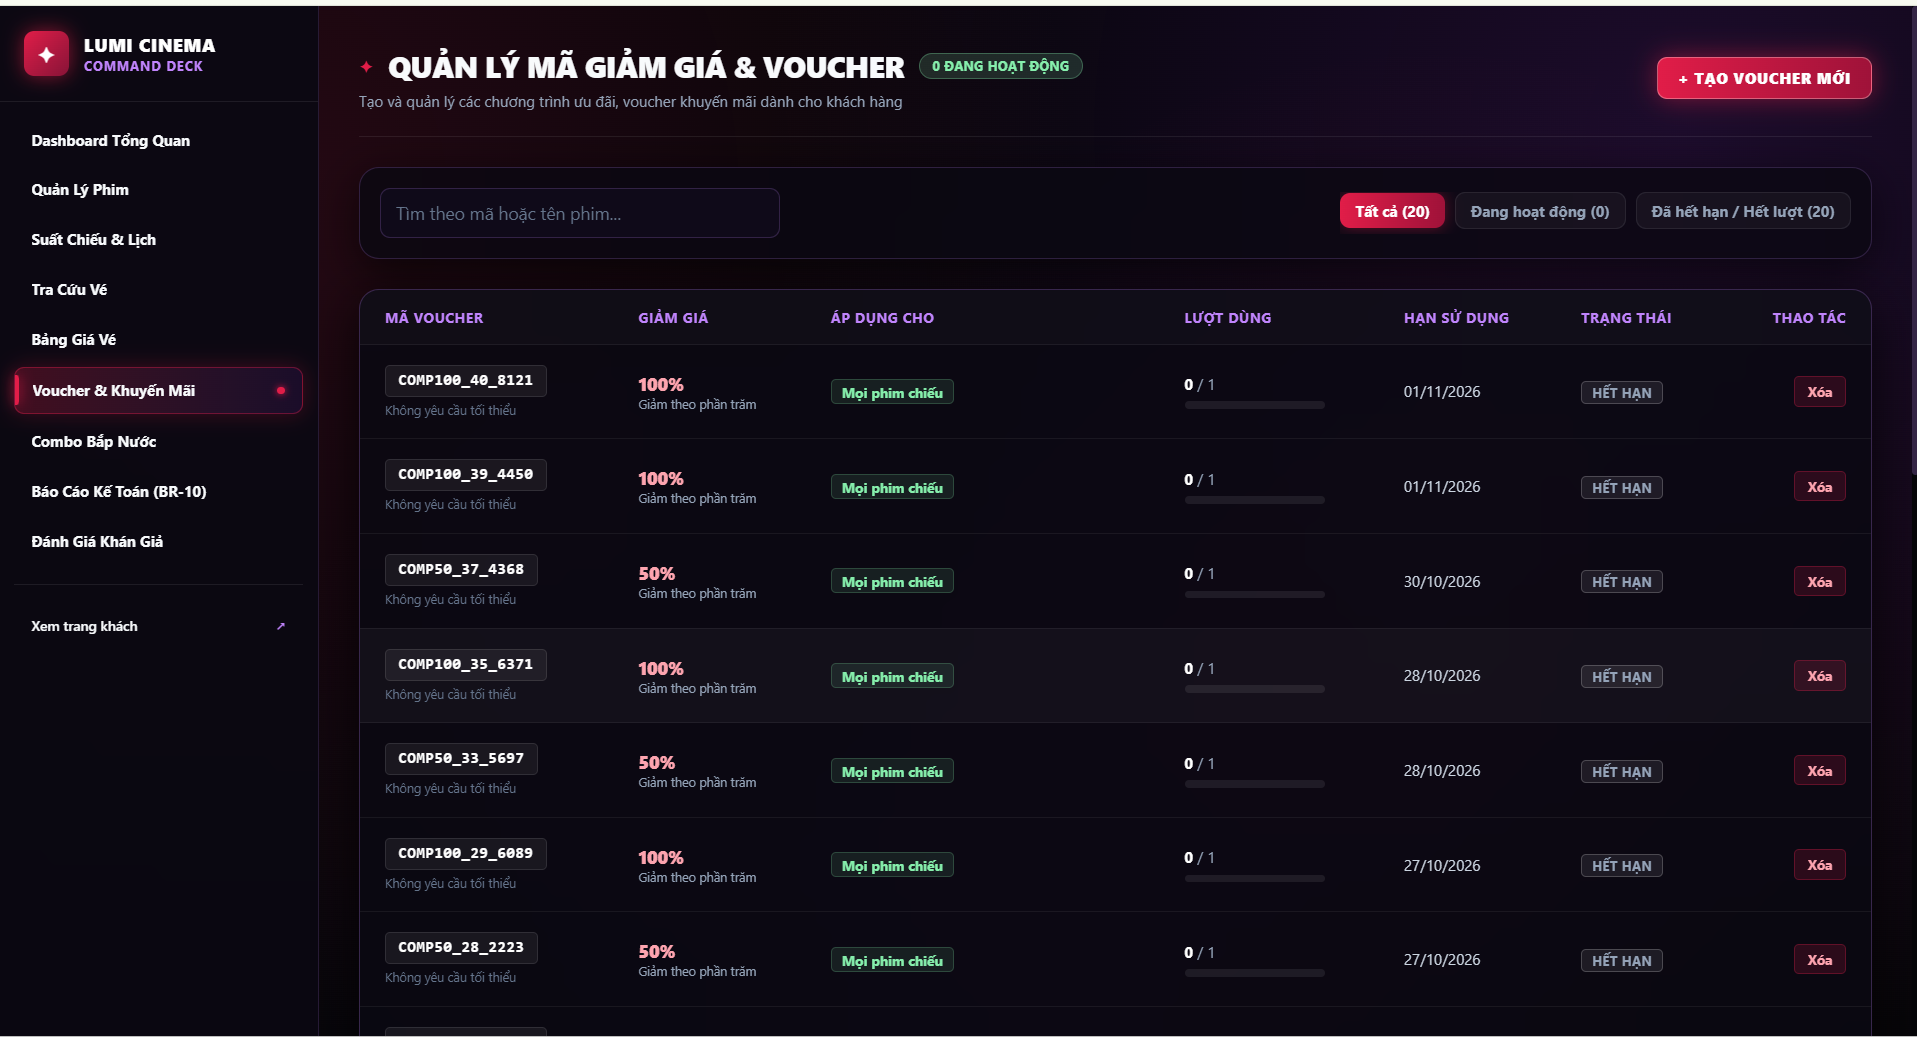
\includegraphics[width=\textwidth,height=0.55\textheight,keepaspectratio]{images/ui/3.23_admin_vouchers.png}
  \caption{Giao diện Quản lý Mã Giảm Giá \& Voucher (/admin/vouchers)}
  \label{fig:ui_3_23}
\end{figure}

\subsection{Giao diện Báo cáo Doanh thu Kế toán (BR-10)}
\begin{figure}[H]
  \centering
  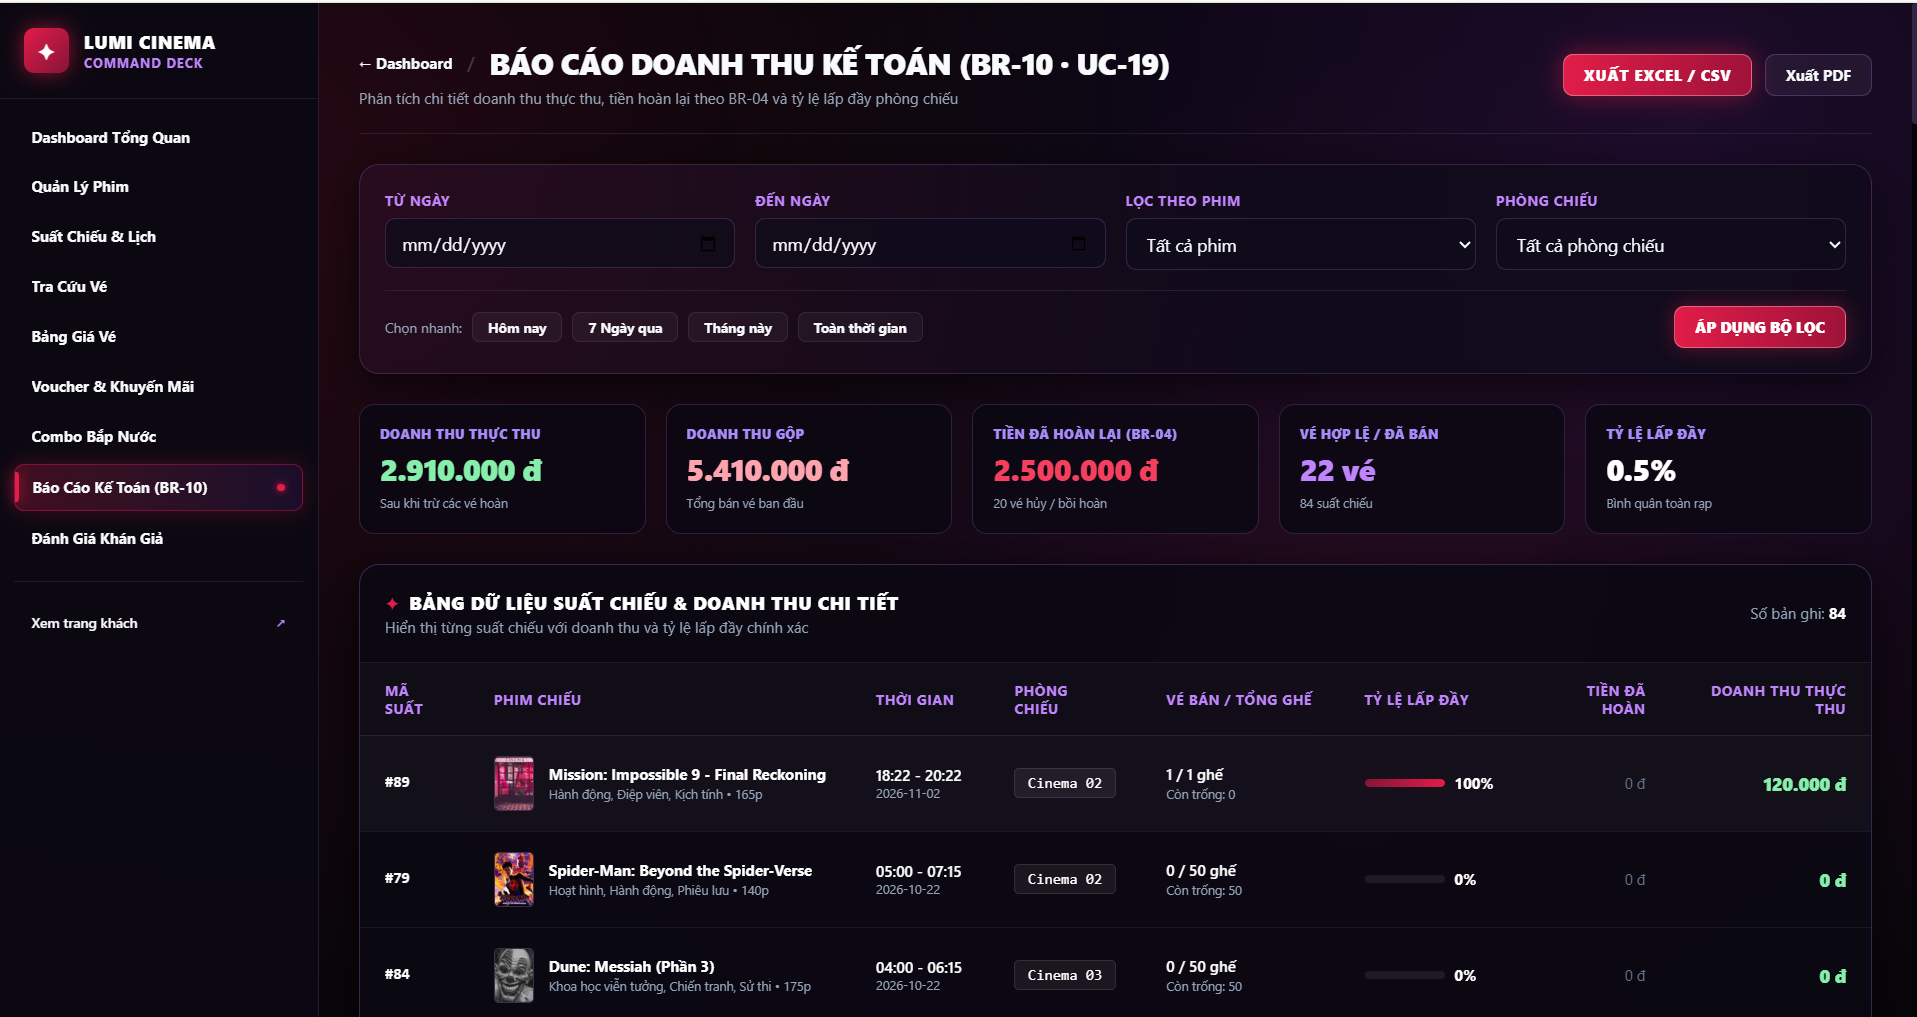
\includegraphics[width=\textwidth,height=0.55\textheight,keepaspectratio]{images/ui/3.24_admin_reports.png}
  \caption{Giao diện Báo cáo Doanh thu Kế toán BR-10 (/admin/reports)}
  \label{fig:ui_3_24}
\end{figure}

\subsection{Giao diện Kiểm duyệt Đánh giá \& Bình luận}
\begin{figure}[H]
  \centering
  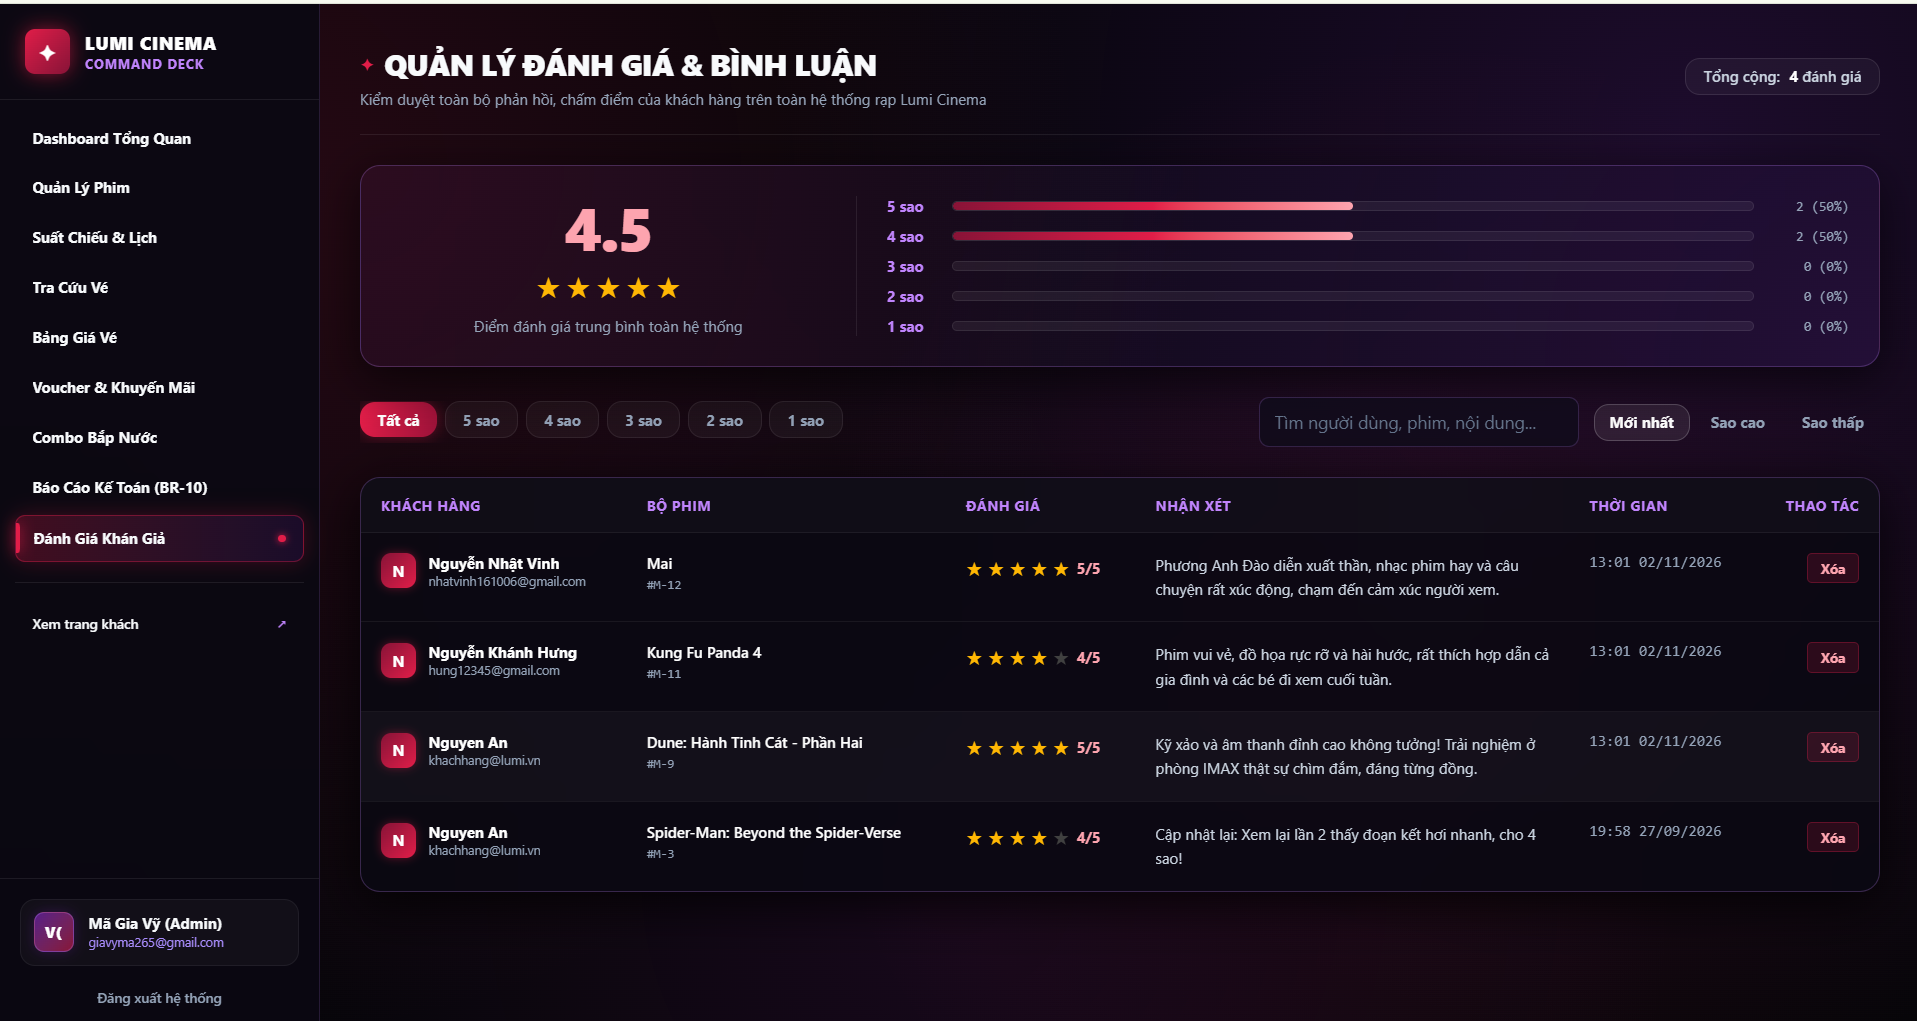
\includegraphics[width=\textwidth,height=0.55\textheight,keepaspectratio]{images/ui/3.25_admin_reviews.png}
  \caption{Giao diện Quản lý Đánh giá Khán giả (/admin/reviews)}
  \label{fig:ui_3_25}
\end{figure}
